% Copied from GitHub: https://github.com/piazzai/arguelles

\documentclass[compress,12pt]{beamer}

\usetheme[sans]{Arguelles}
\usepackage[german]{babel}
\usepackage{textcomp}
\usepackage[utf-8]{inputenc}
\usepackage[T1]{fontenc}


\title{Zwischenergebnisse}
\subtitle{Bachelorarbeit \textit{r/ChangeMyView} Visualisation}
\event{}
\date{}
\author{Christiane Gütter}
\institute{Bauhaus Universität Weimar}

\begin{document}

    \frame[plain]{\titlepage}

%    \begin{frame}[plain]
%        \frametitle{Themen}
%        \begin{enumerate}
%            \item Einführung in das Thema
%            \item Übersicht grundliegendes Paper
%            \item Daten
%            \begin{enumerate}
%                \item Aufbau
%                \item Verarbeitung
%            \end{enumerate}
%            \item Erste potentielle Fragestellungen
%            \item Erste Ergebnisse
%            \begin{enumerate}
%                \item Erste Visualisierungen
%                \item Vergleiche mit Ergebnissen aus Paper
%            \end{enumerate}
%            \item Nächste Schritte
%        \end{enumerate}
%    \end{frame}

    \Section{Einfuehrung}
    \begin{frame}[plain,standout]
        \centering
        \textbf{EINFÜHRUNG}
    \end{frame}

    \begin{frame}{r/ChangeMyView}
        \begin{itemize}
            \item Subreddit, also ein Forum der großen Social Media Seite Reddit.com
            \item Prinzip:
            \begin{itemize}
                \item OP beschreibt Meinung über ein Thema mit Begründung
                \item Commenters geben (hoffentlich) überzeugende Gegenmeinungen
                \item Vergabe von sog.\ Deltas ($\Delta$\rq{}s) durch OP an überzeugende Gegenargumente
            \end{itemize}
            \item gute Eignung zur Analyse, wegen einfacher \lq\lq{}Messung\rq\rq{} der Überzeugungskraft von Argumenten
        \end{itemize}
    \end{frame}

    \begin{frame}[plain]
        \frametitle{r/ChangeMyView}
        \begin{figure}
            \centering
            
\includegraphics[width=\textwidth]{../images/cmv-example-main-page}
            \caption{Frontpage des Subreddits}
            \label{fig:frontpage}
        \end{figure}
    \end{frame}

    \begin{frame}[plain]
        \frametitle{r/ChangeMyView}
        \begin{columns}
            \begin{column}{0.5\textwidth}
                
\includegraphics[width=\columnwidth]{../images/cmv-example-op}
            \end{column}
            \begin{column}{0.5\textwidth}
                
\includegraphics[width=\columnwidth]{../images/cmv-example-thread}
            \end{column}
        \end{columns}
    \end{frame}

    \Section{Zugrundeliegende Daten}
    \begin{frame}[plain,standout]
        \centering
        \textbf{ZUGRUNDELIEGENDE DATEN}
    \end{frame}

    \begin{frame}
        \frametitle{Inhalt}
        {\small
            \begin{quote}
                \lq\lq{}Previous research on argumentation in online discussions has largely focused on \textbf{examining individual comments} and neglected the interactive nature of discussions.
                [\ldots] However, because it is intuitively necessary for dialogical argumentation to address the opposing viewpoints, we extend this model by \textbf{clustering type sequences into different argument arrangement patterns}, thereby \textbf{representing discussions as sequences of these patterns}.
                These sequences of patterns are a \textbf{symbolic representation of argumentation strategies} that capture the overall structure of discussions.[\ldots]\rq\rq{}
            \end{quote}}
    \end{frame}

    \begin{frame}
        \frametitle{Inhalt}
        \begin{itemize}
            \item neuer Ansatz zum Erkennen von argumentativeness
            \item Taggen von Posts und Kommentaren mit sog.\ ADU (argumentative discourse unit) types auf Wortgruppenebene
            \begin{itemize}
                \item \textbf{Value:} \lq\lq{}[\ldots] proposition that refers to subjective value judgments [\ldots]\rq\rq{}
                \item \textbf{Fact:} \lq\lq{}[\ldots] proposition describing objective facts that can be verified using objective evidence [\ldots]\rq\rq{}
                \item \textbf{Policy:} \lq\lq{}[\ldots] a specific course of action to be taken or what should be done [\ldots]\rq\rq{}
                \item \textbf{Testimony:} \lq\lq{}[\ldots]objective proposition related to the author’s personal state or experience [\ldots]\rq\rq{}
                \item \textbf{Rhetorical Statement:} \lq\lq{}[\ldots] subjective value judgment by expressing figurative phrases, emotions, or rhetorical questions [\ldots]\rq\rq{}
            \end{itemize}
        \end{itemize}
    \end{frame}
    
    \begin{frame}[plain]
        \frametitle{Inhalt}
        \begin{figure}
            \centering
            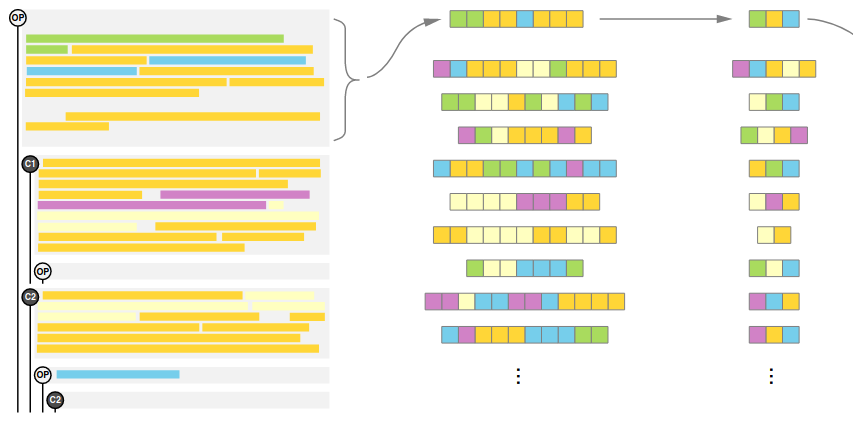
\includegraphics[width=\textwidth]{../images/sequencing-part-1}
            \caption{Weg vom Kommentar zur Sequenz}
            \label{fig:comment-to-sequence}
        \end{figure}
    \end{frame}

    \begin{frame}
        \frametitle{Inhalt}
        \begin{figure}
            \centering
            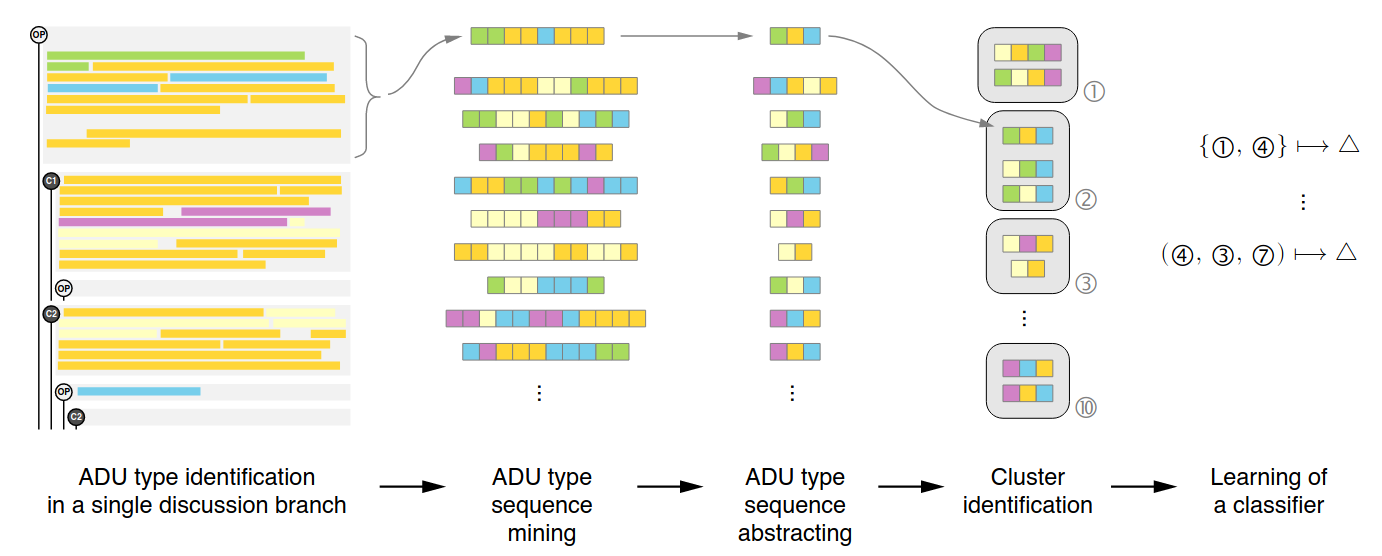
\includegraphics[width=\textwidth]{../images/sequencing}
            \caption{Modeling the overall strategy of two discussion branches as flows of ADU type arrangements per its original post and comments. [...]}
            \label{fig:adu-sequencing}
        \end{figure}
    \end{frame}

    \begin{frame}{Daten}
        \begin{itemize}
            \item \textasciitilde 34k Branches (ein Pfad von der Wurzel (OP) bis zu einem Leaf-Kommentar)
            \item \textasciitilde 3k Branches, die ein Delta erhalten haben
            \item \textrightarrow{} Visualisierung aller Threads schwierig
            \item Aufteilung in Polyloge und Dialoge
        \end{itemize}
    \end{frame}

    \begin{frame}{Aufbau}
        \begin{itemize}
            \item Auflistung in JSON Files
            \item einzelnes File = eine einzelne Unterhaltung
            \item Filename = eindeutige ID des OP, Threads aufsteigend nummeriert
        \end{itemize}
    \end{frame}

    \begin{frame}[plain]
        \frametitle{Aufbau}
        \begin{figure}
            \centering
            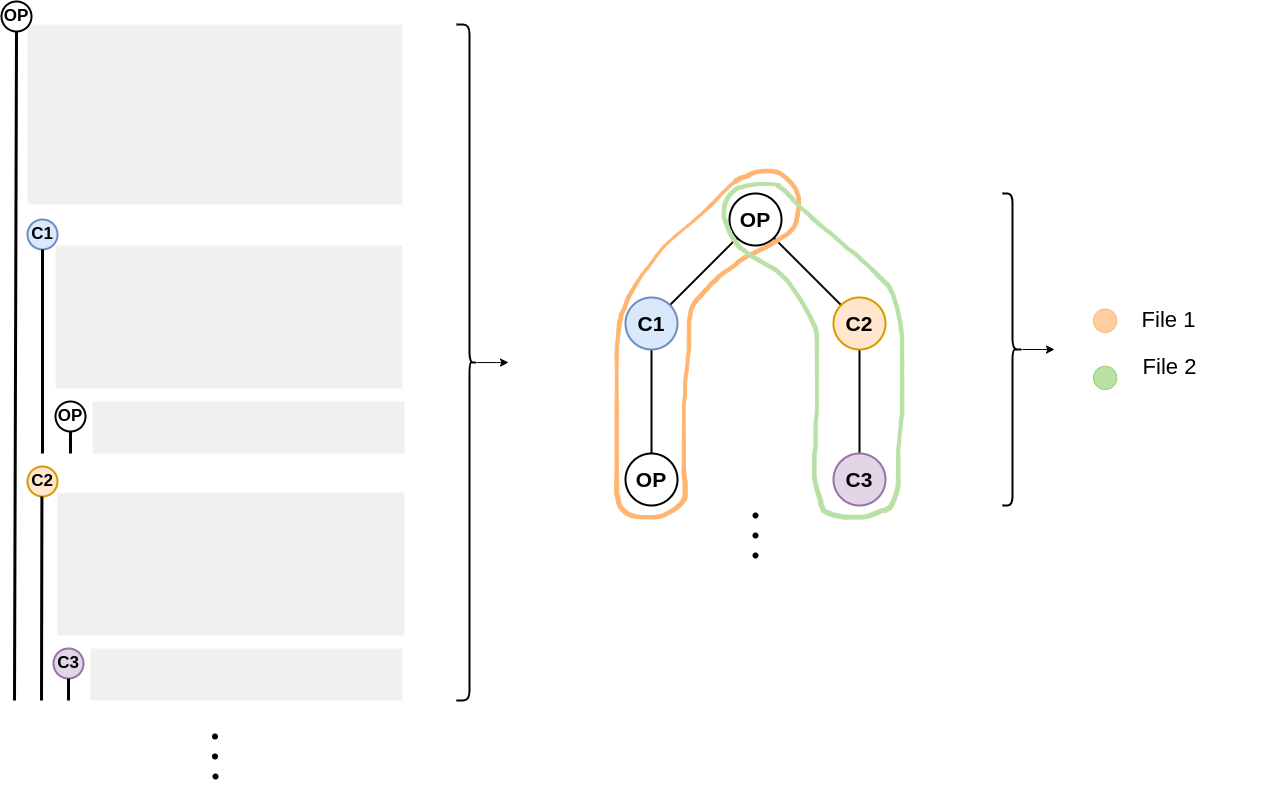
\includegraphics[width=0.9\textwidth]{../images/data-files-structure}
            \caption{Visuelle Aufteilung der Files und deren Inhalt angefangen vom Reddit Post}
            \label{fig:data-structure}
        \end{figure}
    \end{frame}

    \begin{frame}[plain]
        \frametitle{Aufbau}
        \begin{figure}
            \centering
            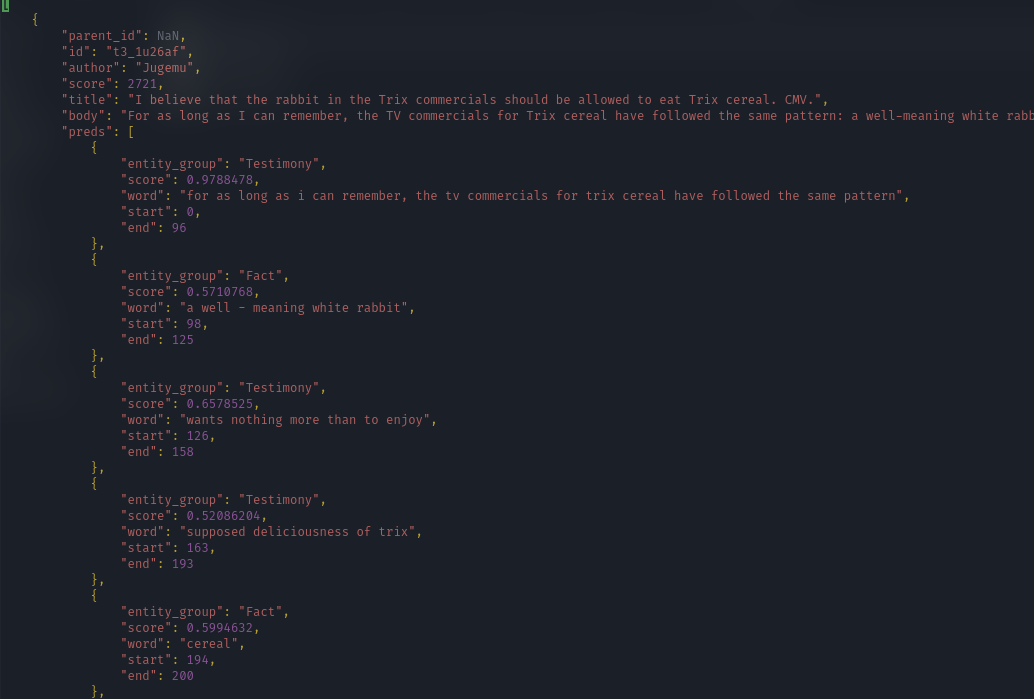
\includegraphics[width=0.9\textwidth]{../images/single-file-example}
            \caption{Beispielinhalt eines einzelnen Files}
            \label{fig:single-file-example}
        \end{figure}
    \end{frame}

    \begin{frame}{Aufbau}
        \begin{itemize}
            \item Cluster in eigenen Files
            \item OP Cluster und Comment Cluster getrennt
            \item JSONL Files: eine Zeile = \texttt{\{comment\_id, abstract\_adus, sequence, cluster\}}
        \end{itemize}
    \end{frame}

    \begin{frame}[plain]
        \frametitle{Aufbau}
        \begin{figure}
            \centering
            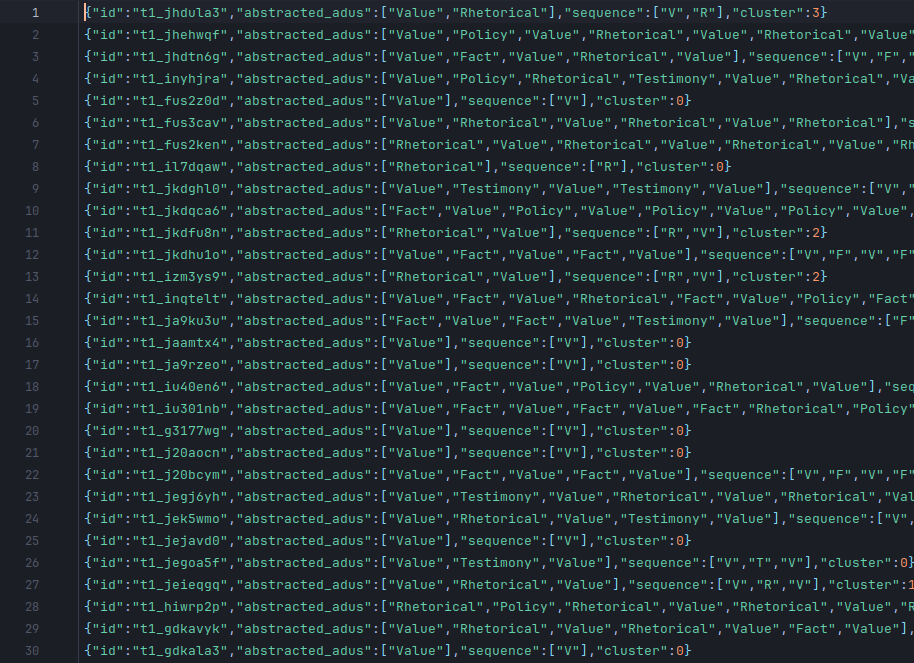
\includegraphics[width=0.9\textwidth]{../images/cluster-file-example}
            \caption{Ausschnitt aus einem Cluster File}
            \label{fig:cluster-file-example}
        \end{figure}
    \end{frame}

%    \begin{frame}{Verarbeitung}
%        \begin{itemize}
%            \item per Python Script, Darstellung mit d3 und JS
%            \item Sortieren aller Files mit der gleichen ID (einem Baum angehörig) in einen Unterordner (ID als Name)
%            \item Iterieren über alle Unterordner und den enthaltenen Files
%            \item Aufbauen eines großen JSON File (Array aus Arrays) für das Verarbeiten in d3 mit den nötigen Daten
%            \item Generieren verschiedener CSV Files für verschiedene Visualisierungen
%        \end{itemize}
%    \end{frame}
%
%    \begin{frame}[plain]
%        \frametitle{Verarbeitung}
%        \begin{columns}
%            \begin{column}{0.5\textwidth}
%                \begin{figure}
%                    \centering
%                    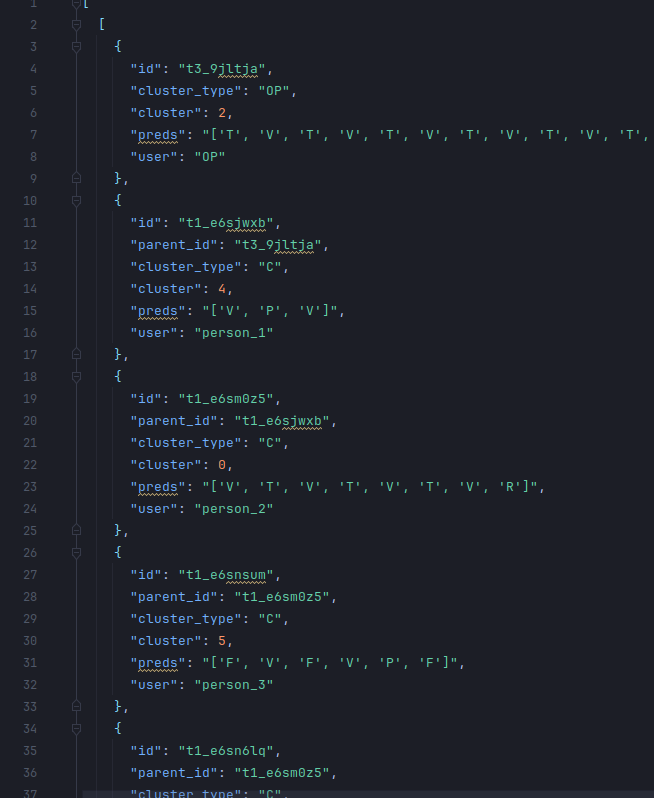
\includegraphics[width=\textwidth]{../images/json-file-example}
%                    \caption{Beispiel eines großen JSON Files}
%                    \label{fig:json-file-example}
%                \end{figure}
%            \end{column}
%            \begin{column}{0.5\textwidth}
%                \begin{figure}
%                    \centering
%                    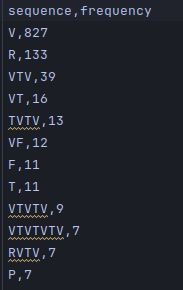
\includegraphics[width=0.8\textwidth]{../images/csv-file-example}
%                    \caption{Beispiel eines CSV Files (Anzahl aller Sequenzen in C1)}
%                    \label{fig:csv-file-example}
%                \end{figure}
%            \end{column}
%        \end{columns}
%    \end{frame}

    \Section{Fragestellungen}
    \begin{frame}[plain,standout]
        \centering
        \textbf{FRAGESTELLUNG}
    \end{frame}

    \begin{frame}
        \frametitle{Ergebnisse \& Erkenntnisse}
        \textit{Haupterkenntnis:} Nach Training ist Language Model/Transformer wesentlich besser im Erkennen von stärkeren Argumentationen/Argumentationssträngen als z.B.\ BERT-like Language Models \\
        \vspace{1pc}
        \textit{weitere Erkenntnisse:} Optimum ist bei 2--3 Posts per Branch für ein Delta, kürzere Unterhaltungen erhielten eher ein Delta als längere
    \end{frame}

    \begin{frame}
        \frametitle{Ergebnisse \& Erkenntnisse}
        Was uns aufgefallen ist:
        \begin{itemize}
            \item Layout der Webseite: 2--3 Kommentare werden angezeigt, bis man den Rest aufklappen muss
            \item Zeitlicher Einfluss (Vergabe von Deltas hört irgendwann auf)
            \item Fülle der Kommentare (OP kann nicht alle Kommentare lesen und auf sie eingehen)
        \end{itemize}
    \end{frame}

    \begin{frame}{Problematik}
        \item offene Fragen:
        \begin{itemize}
            \item Abstraktion von Sequenzen und Zusammenfassung in Clustern \textrightarrow{} Was ist eigentlich in den Clustern drin?
            \item Sind die representativen Sequenzen aus dem Paper tatsächlich representativ?
            \item Welche Muster gibt es in den Argumentationsstrukturen?
            Kann man als Mensch diese als \lq\lq{}überzeugend\rq\rq{} oder \lq\lq{}nicht überzeugend\rq\rq{} einordnen?
            \item Welchen Einfluss hat die (Gesamt-)Diskussion auf die finale Vergabe des Deltas?
        \end{itemize}
    \end{frame}

%    \begin{frame}{Nicht im Fokus oder Scope}
%        \begin{itemize}
%            \item Untersuchung des zeitlichen Einflusses und OP Verhalten
%            \item nähere Untersuchung der User \textrightarrow{} mit den vorhandenen Informationen schwierig, von anderem Webis Paper untersucht
%            \item Vergleiche zwischen Delta und nicht-Delta durch große Datenmengen schwierig(er)
%        \end{itemize}
%    \end{frame}

    \begin{frame}{Im Fokus}
        \begin{itemize}
            \item Strukturelle Untersuchung der Threads/Bäume
            \item Visuelle und statistische Untersuchung des Inhalts von Clustern:
            \begin{itemize}
                \item Welche Sequenzen kommen vor und wie oft?
                \item In welchen Anteilen sind die ADU Types enthalten?
                \item Welche ADU Types folgen wie oft auf andere?
            \end{itemize}
            \item Aufbau der Diskussionen:
            \begin{itemize}
                \item Welche Cluster folgen oft auf andere in \lq\lq{}überzeugenden\rq\rq{} Diskussionen?
            \end{itemize}
        \end{itemize}
    \end{frame}

%    \begin{frame}{Brainstorming}
%        \begin{itemize}
%            \item Untersuchen der User und deren Einfluss:
%            \begin{itemize}
%                \item in Polylogen: ist Beteiligung von mehr Leuten effektiver?\ Polyloge vs.\ Dialoge?
%                \item Sind viele kurze Antworten effektiver als weniger lange?
%                \item Bekommen User mit schon vielen Deltas potientiell noch mehr Deltas?
%                \item In welchen Clustern kommen welche User vor?
%                \item Wie hat die Aktivität von OP die Ergebnisse beeinflusst?\ (Zeit, Menge der Antworten, etc.)
%            \end{itemize}
%            \item Einfluss des Layouts der Webseite auf die Ergebnisse
%        \end{itemize}
%    \end{frame}

    \Section{Erste Visualisierungen}
    \begin{frame}[plain,standout]
        \centering
        \textbf{ERSTE VISUALISIERUNGEN}
    \end{frame}

    \begin{frame}{Threads}
        \begin{figure}
            \centering
            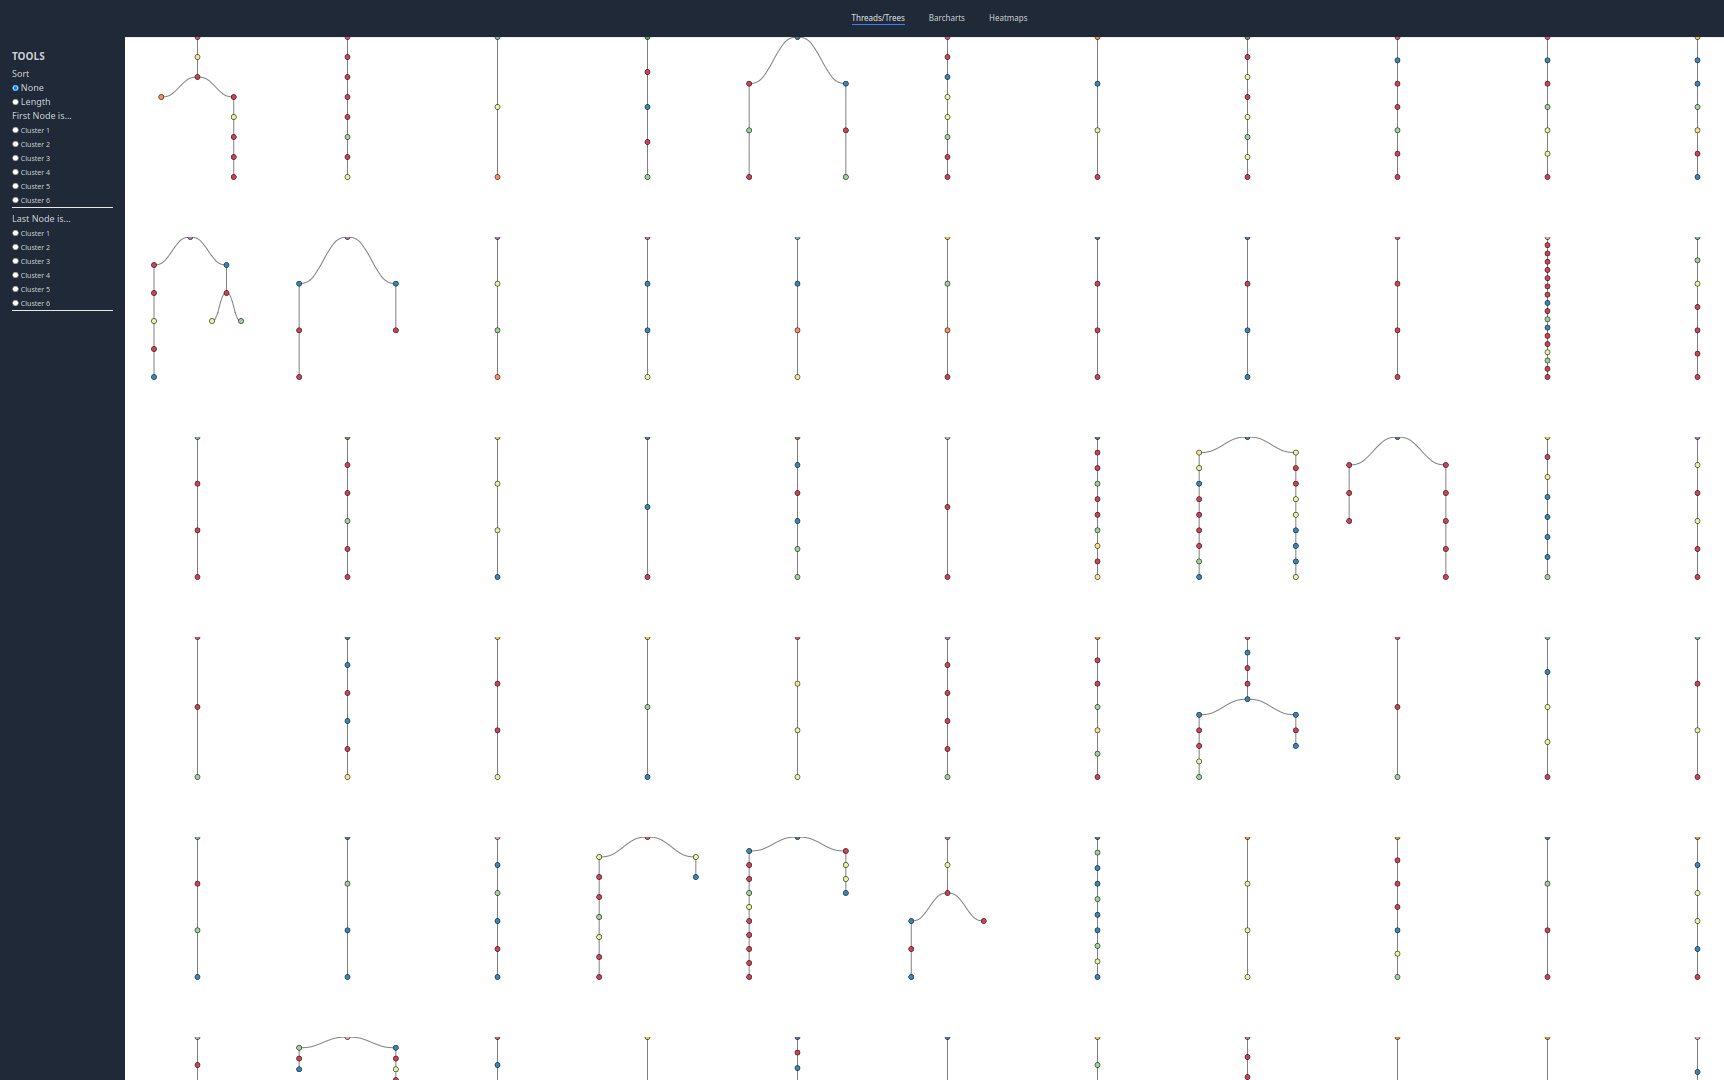
\includegraphics[width=\textwidth]{../images/threads-example}
            \caption{Thread Visualisierung zur strukturellen Untersuchung (Polyloge)}
            \label{fig:thread-example}
        \end{figure}
    \end{frame}

    \begin{frame}{Threads}
        \begin{figure}
            \centering
            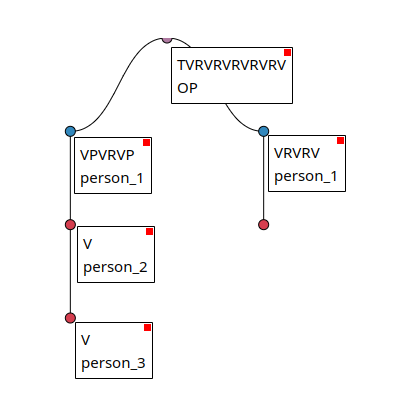
\includegraphics[width=0.55\textwidth]{../images/single-thread-example}
            \caption{Thread Visualisierung zur strukturellen Untersuchung (Polyloge)}
            \label{fig:single-thread-example}
        \end{figure}
    \end{frame}

    \begin{frame}{Barcharts + Piecharts}
        \begin{figure}
            \centering
            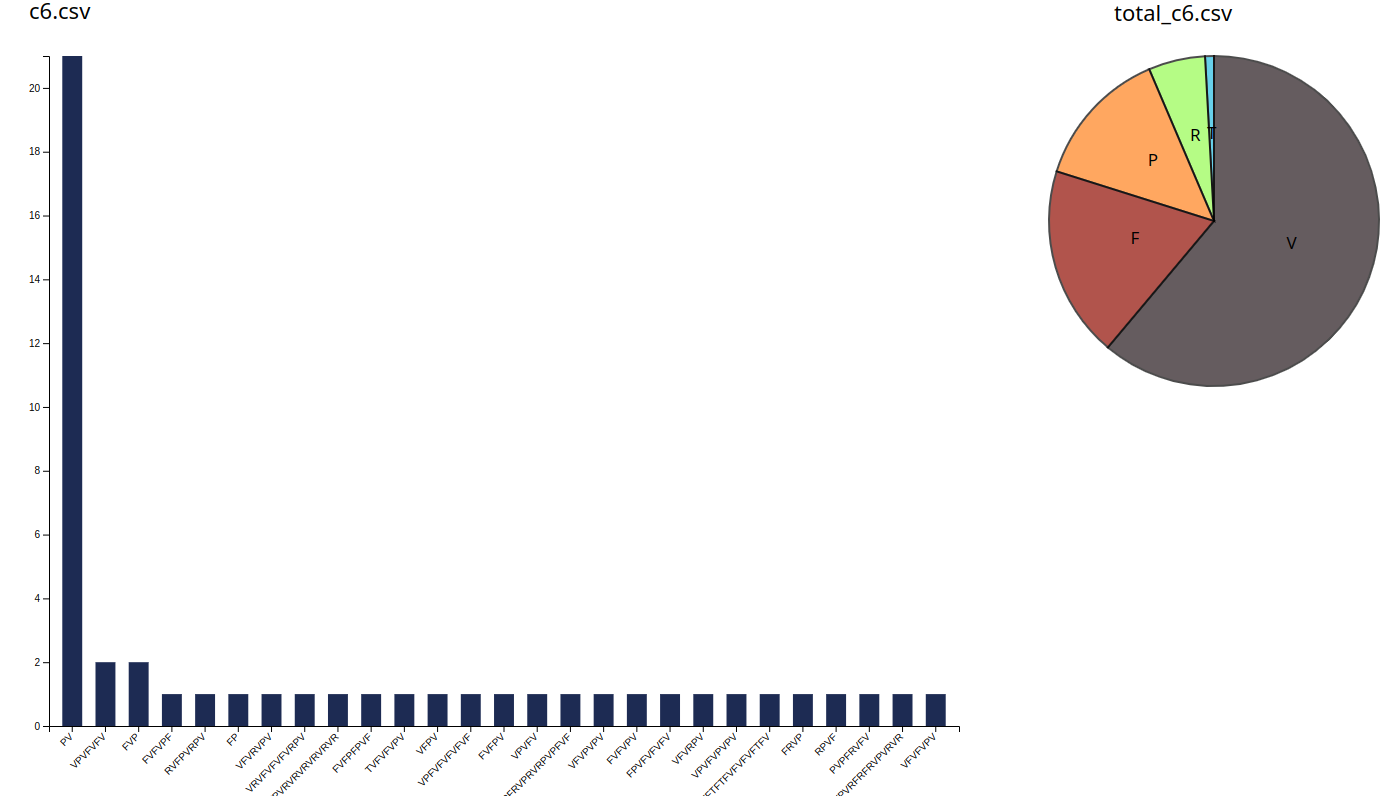
\includegraphics[width=0.9\textwidth]{../images/bar-pie-charts-example}
            \caption{Bar- und Piecharts zur Untersuchung des Aufbaus der einzelnen Cluster (hier C6)}
            \label{fig:bar-pie-charts-example}
        \end{figure}
    \end{frame}

    \begin{frame}{Heatmaps + Bars}
        \begin{figure}
            \centering
            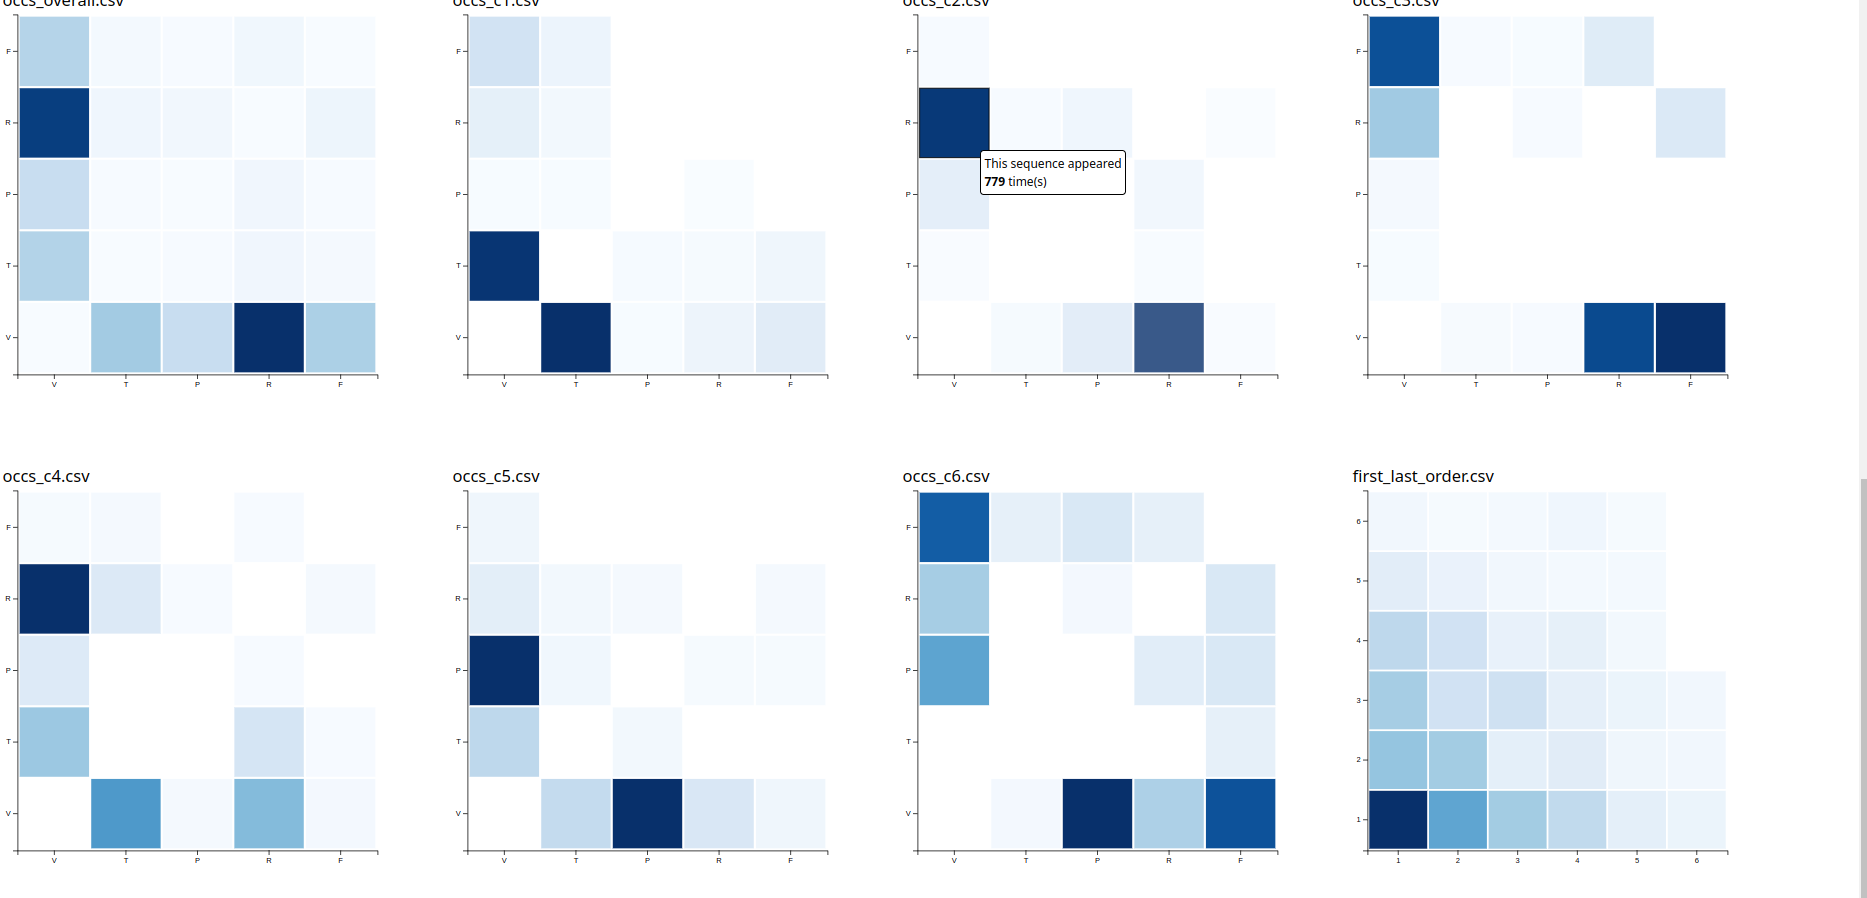
\includegraphics[width=0.9\textwidth]{../images/heatmaps-example}
            \caption{Heatmaps zur Untersuchung von strukturellen Eigenschaften der Cluster}
            \label{fig:heatmaps-example}
        \end{figure}
    \end{frame}

    \begin{frame}{Heatmaps + Bars}
        \begin{figure}
            \centering
            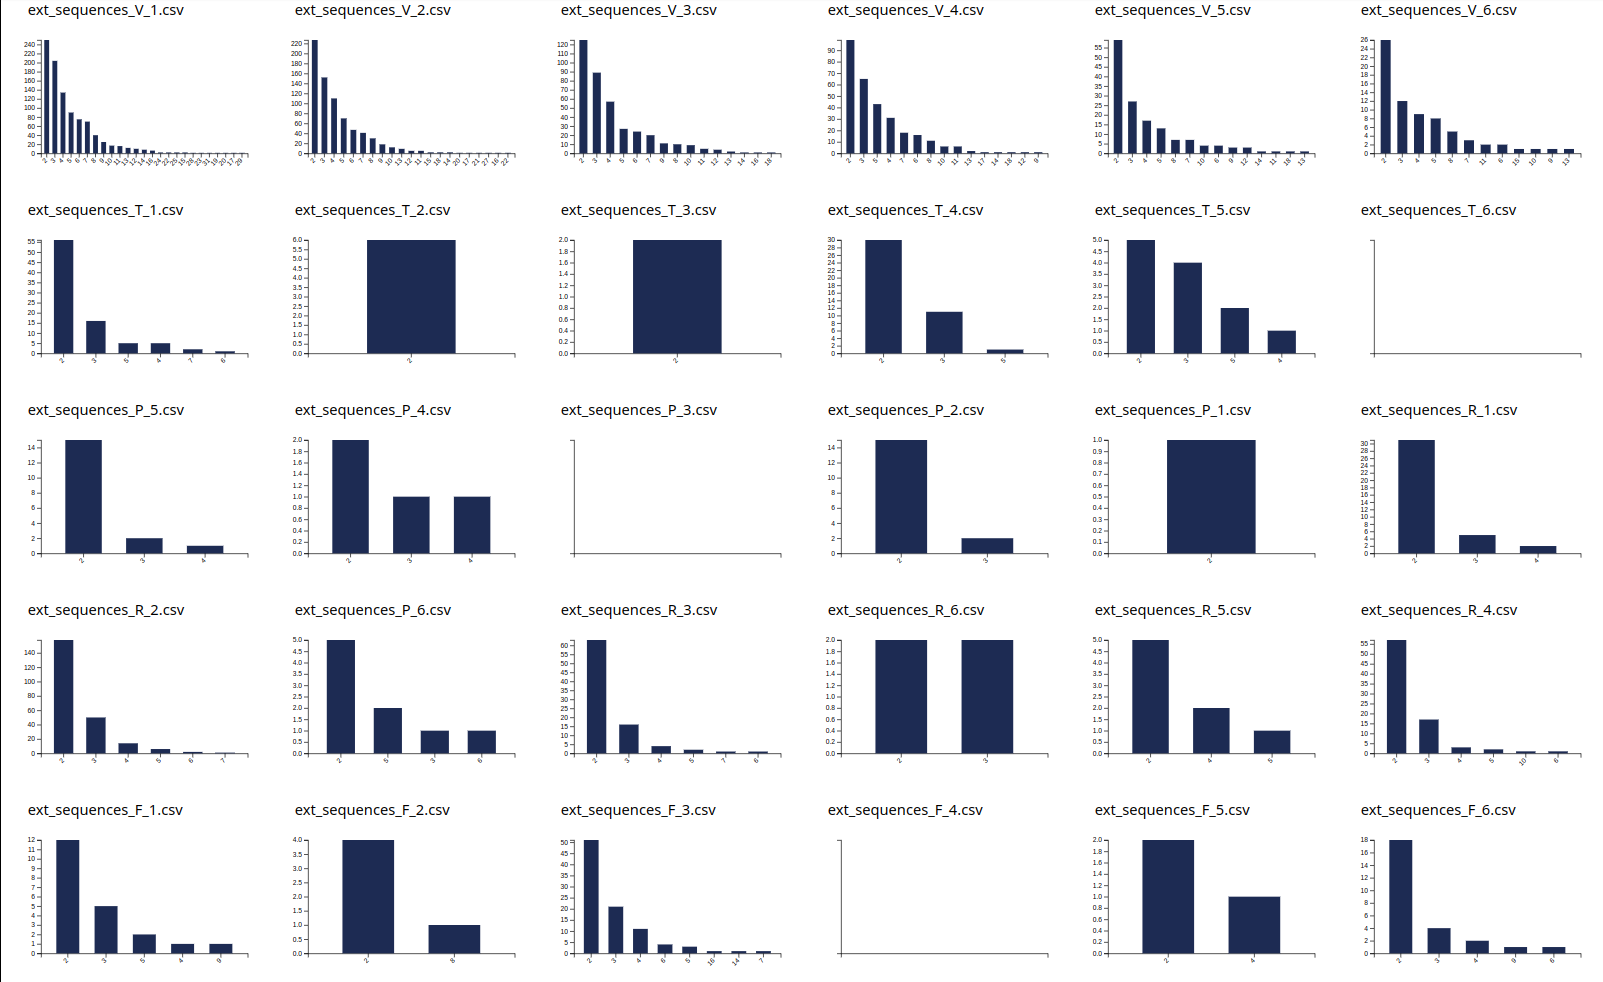
\includegraphics[width=0.9\textwidth]{../images/heatmap-bars-example}
            \caption{Barcharts zur Untersuchung von aufeinanderfolgenen gleichen ADU Types (werden den Heatmaps hinzugefügt oder mit entcoded)}
            \label{fig:heatmap-bars-example}
        \end{figure}
    \end{frame}

    \Section{Erste Ergebnisse}
    \begin{frame}[plain,standout]
        \centering
        \textbf{ERSTE ERGEBNISSE}
    \end{frame}

    \begin{frame}{Einsichten}
        \begin{itemize}
            \item Values sind der am meisten vorkommende ADU Type
            \item ein paar Sequenzen pro Cluster kommen sehr oft vor, der Großteil nur noch wenig oder sogar nur einmal
            \item Cluster unterscheiden sich sichtbar im Aufbau
            \item Muster im Threadaufbau = kurz, simpel, wenig verzweigt
        \end{itemize}
    \end{frame}

    \Section{Naechste Schritte}
    \begin{frame}[plain,standout]
        \centering
        \textbf{NÄCHSTE SCHRITTE}
    \end{frame}

    \begin{frame}{Nächste Schritte}
        \begin{itemize}
            \item Einsichten der Heatmaps weiter untersuchen, Visualisierung der Cluster-Struktur weiter ausbauen
            \item Vergleich zwischen Delta Threads und (Subset von) nicht-Delta Threads auf Cluster Ebene
            \item Vergleich zwischen Clustern auf ADU-Type Ebene
        \end{itemize}
    \end{frame}

    \End

    \begin{frame}[plain,standout]
        \centering
        \textbf{FRAGEN \& DISKUSSION}
    \end{frame}

\end{document}
